% \iffalse meta-comment
%
% Copyright (C) 2018--2023 by Xiangdong Zeng <xdzeng96@gmail.com>
%
% This work may be distributed and/or modified under the
% conditions of the LaTeX Project Public License, either
% version 1.3c of this license or (at your option) any later
% version. The latest version of this license is in:
%
%   http://www.latex-project.org/lppl.txt
%
% and version 1.3 or later is part of all distributions of
% LaTeX version 2005/12/01 or later.
%
% This work has the LPPL maintenance status `maintained'.
%
% The Current Maintainer of this work is Xiangdong Zeng.
%
% \fi

%*********************************************************************
% fduthesis: 复旦大学论文模板
% 2023-05-27 v0.9a
%
% 重要提示：
%   1. 请确保使用 UTF-8 编码保存
%   2. 请使用 XeLaTeX 或 LuaLaTeX 编译
%   3. 请仔细阅读用户文档
%   4. 修改、使用、发布本文档请务必遵循 LaTeX Project Public License
%   5. 不需要的注释可以尽情删除
%*********************************************************************

\documentclass[type=master]{fduthesis}
% 模板选项：
%   type = doctor|master|bachelor  论文类型，默认为本科论文
%   oneside|twoside                论文的单双面模式，默认为 twoside
%   draft = true|false             是否开启草稿模式，默认关闭
% 带选项的用法示例：
%   \documentclass[oneside]{fduthesis}
%   \documentclass[twoside, draft=true]{fduthesis}
%   \documentclass[type=bachelor, twoside, draft=true]{fduthesis}

\fdusetup{
  % 参数设置
  % 允许采用两种方式设置选项：
  %   1. style/... = ...
  %   2. style = { ... = ... }
  % 注意事项：
  %   1. 不要出现空行
  %   2. “=” 两侧的空格会被忽略
  %   3. “/” 两侧的空格不会被忽略
  %   4. 请使用英文逗号 “,” 分隔选项
  %
  % style 类用于设置论文格式
  style = {
    % font = times,
    % 西文字体（包括数学字体）
    % 允许选项：
    %   font = garamond|libertinus|lm|palatino|times|times*|none
    %
    % cjk-font = none,
    % cjk-font = fandol,
    % 中文字体
    % 允许选项：
    %   cjk-font = adobe|fandol|founder|mac|sinotype|sourcehan|windows|none
    %
    % 注意：
    %   1. 中文字体设置高度依赖于系统。各系统建议方案：
    %        windows：cjk-font = windows
    %        mac：    cjk-font = mac
    %        linux：  cjk-font = fandol（默认值）
    %   2. 除 fandol 和 sourcehan 外，其余字体均为商用字体，请注意版权问题
    %   3. 但 fandol 字体缺字比较严重，而 sourcehan 没有配备楷体和仿宋体
    %   4. 这里中西文字体设置均注释掉了，即使用默认设置：
    %        font     = times
    %        cjk-font = fandol
    %   5. 使用 font = none / cjk-font = none 关闭默认字体设置，需手动进行配置
    %
    % font-size = -4,
    % 字号
    % 允许选项：
    %   font-size = -4|5
    %
    % fullwidth-stop = catcode,
    % 是否把全角实心句点 “．” 作为默认的句号形状
    % 允许选项：
    %   fullwidth-stop = catcode|mapping|false
    % 说明：
    %   catcode   显式的 “。” 会被替换为 “．”（e.g. 不包括用宏定义保存的 “。”）
    %   mapping   所有的 “。” 会被替换为 “．”（使用 LuaLaTeX 编译则无效）
    %   false     不进行替换
    %
    footnote-style = xits,
    % 脚注编号样式
    % 允许选项：
    %   footnote-style = plain|libertinus|libertinus*|libertinus-sans|
    %                    pifont|pifont*|pifont-sans|pifont-sans*|
    %                    xits|xits-sans|xits-sans*
    % 默认与西文字体保持一致
    %
    % hyperlink = color,
    % 超链接样式
    % 允许选项：
    %   hyperlink = border|color|none
    %
    % hyperlink-color = default,
    % 超链接颜色
    % 允许选项：
    %   hyperlink-color = default|classic|material|graylevel|prl
    %
    bib-backend = bibtex,
    % 参考文献支持方式
    % 允许选项：
    %   bib-backend = bibtex|biblatex
    %
    % bib-style = numerical,
    % 参考文献样式
    % 允许选项：
    %   bib-style = author-year|numerical|<其他样式>
    % 说明：
    %   author-year  著者—出版年制
    %   numerical    顺序编码制
    %   <其他样式>   使用其他 .bst（bibtex）或 .bbx（biblatex）格式文件
    %
    % cite-style = {},
    % 引用样式
    % 默认为空，即与参考文献样式保持一致
    % 仅适用于 biblatex；如要填写，需保证相应的 .cbx 格式文件能被调用
    %
    bib-resource = {main.bib},
    % 参考文献数据源
    % 可以是单个文件，也可以是用英文逗号 “,” 隔开的一组文件
    % 如果使用 biblatex，则必须明确给出 .bib 后缀名
    %
    % logo = {fudan-name.pdf},
    % 封面中的校名图片
    % 模版已自带，通常不需要额外配置
    %
    % logo-size = {0.5\textwidth},      % 只设置宽度
    % logo-size = {{}, 3cm},            % 只设置高度
    % logo-size = {8cm, 3cm},           % 设置宽度和高度
    % 设置校名图片的大小
    % 通常不需要调整
    %
    % declaration-page = {declaration.pdf},
    % 插入扫描版的声明页 PDF 文档
    % 默认使用预定义的声明页，但不带签名
    %
    % auto-make-cover = true
    % 是否自动生成论文封面（封一）、指导小组成员名单（封二）和声明页（封三）
    % 除非特殊需要（e.g. 不要封面），否则不建议设为 false
  },
  %
  % info 类用于录入论文信息
  info = {
    title = {量子顺磁体的自旋能斯特效应},
    % 中文标题
    % 长标题建议使用 “\\” 命令手动换行（不是指在源文件里输入回车符，当然
    % 源文件里适当的换行可以有助于代码清晰）：
    %   title = {最高人民法院、最高人民检察院关于适用\\
    %            犯罪嫌疑人、被告人逃匿、死亡案件违法所得\\
    %            没收程序若干问题的规定},
    %
    title* = {Spin Nernst effects in quantum paramagnets},
    % 英文标题
    %
    author = {卢博文},
    % 作者姓名
    %
    % author* = {Your name},
    % 作者姓名（英文 / 拼音）
    % 目前不需要填写
    %
    supervisor = {虞跃 \  教授 \& 陈钢 \  教授},
    % 导师
    % 姓名与职称之间可以用 \quad 打印一个空格
    %
    major = {理论物理},
    % 专业
    %
    degree = academic,
    % 学位类型
    % 允许选项：
    %   degree = academic|professional
    % 说明：
    %   academic      学术学位
    %   professional  专业学位
    %
    department = {物理学系},
    % 院系
    %
    student-id = {21110190043},
    % 作者学号
    %
    date = {2025 年 5 月 24 日},
    % 日期
    % 注释掉表示使用编译日期
    %
    % secret-level = ii,
    % 密级
    % 允许选项：
    %   secret-level = none|i|ii|iii
    % 说明：
    %   none  不显示密级与保密年限
    %   i     秘密
    %   ii    机密
    %   iii   绝密
    %
    % secret-year = {五年},
    % 保密年限
    % secret-level = none 时该选项无效
    %
    instructors = {
      {虞\quad 跃 \quad 教\quad 授},
      {陈\quad 钢 \quad 教\quad 授}
    },
    % 指导小组成员
    % 使用英文逗号 “,” 分隔
    % 如有需要，可以用 \quad 手工对齐
    %
    keywords = {量子顺磁体, 味能斯特效应, 自旋输运，贝里曲率，拓扑自旋输运。},
    % 中文关键词
    % 使用英文逗号 “,” 分隔
    %
    keywords* = {Quantum Paramagnets, Flavor Nernst Effect, Spin Transport, Berry Curvature, Topological Spin Transport.},
    % 英文关键词
    % 使用英文逗号 “,” 分隔
    %
    clc = {O469},
    % 中图分类号
    %
    % jel = {C02},
    % JEL 分类号，仅适用于经济学院等部分院系
  }
}

% 需要的宏包可以自行调用
\usepackage{physics}
\usepackage[colorlinks=true,citecolor=blue,linkcolor=blue,urlcolor=blue]{hyperref}
%\usepackage{bm}
\usepackage{times}
\usepackage{cases}
% \usepackage{wasysym}
\usepackage[version=4]{mhchem}
\usepackage{graphicx}
\usepackage{subfigure}
\usepackage{booktabs}  %provide toprule
\usepackage{multirow}
\usepackage{tikz}
\usepackage[normalem]{ulem}
\usepackage{comment}
\usepackage{lineno}

% 需要的命令可以自行定义
\newcommand{\hilbertH}{\symcal{H}}
\newcommand{\ee}{\symrm{e}}
\newcommand{\ii}{\symrm{i}}
\newcommand{\bm}[1]{\symbf{#1}}

% Hacks
\ExplSyntaxOn
\cs_set_protected:Npn \__fdu_load_cjk_font_fandol:
  {
    \__fdu_setCJKmainfont:nn  { HYShuSongErS.ttf } { BoldFont = HYZhongSongS.ttf }
    \__fdu_setCJKsansfont:n   { HYZhongHeiS.ttf  }
    \__fdu_setCJKmonofont:n   { HYFangSongS.ttf  }
    \__fdu_set_cjk_font_kai:n { HYKaiTiS.ttf     }
  }
\cs_set:Npn \fdu_allow_url_break:
  {
    \cs_set:Npn \UrlBreaks
      {
        \do \. \do \@ \do \\ \do \/ \do \! \do \_ \do \| \do \; \do \>
        \do \] \do \) \do \, \do \? \do \& \do \' \do  + \do \= \do \#
      }
  }
\cs_set_protected:Npn \__fdu_abstract_end:
  {
    \__fdu_keywords:nNn
      { \sffamily \c__fdu_name_keywords_tl \c__fdu_fwid_colon_tl \hspace{ -0.2em } }
      \l__fdu_info_keywords_clist { \c__fdu_fwid_semicolon_tl \hspace{ -0.2em } }
    \__fdu_clc_jel:nn
      { \sffamily \c__fdu_name_clc_tl \c__fdu_fwid_colon_tl }
      { \l__fdu_info_clc_tl }
  }
\cs_set_protected:Npn \__fdu_abstract_en_begin:
  {
    \__fdu_chapter:V \c__fdu_name_abstract_en_tl
    \__fdu_line_spread:n { 1.3 }
  }
\exp_args:Nc \ctex_patch_cmd:Nnn { l@chapter }
  { \vskip 1.0em }
  { \vskip 0.8em }
\ExplSyntaxOff


\graphicspath{{figures/}}

\begin{document}

% 这个命令用来关闭版心底部强制对齐，可以减少不必要的 underfull \vbox 提示，但会影响排版效果
% \raggedbottom

% 前置部分包含目录、中英文摘要以及符号表等
\frontmatter

% 目录
\tableofcontents
% 插图目录
\listoffigures
% 表格目录
% \listoftables

\begin{abstract}
  自旋输运这一新兴领域揭示了量子顺磁体引人注目的潜力，尽管它们缺乏长程磁有序，但却具备展现新奇现象的能力，并为先进技术应用开辟了道路。本论文深入探讨了量子顺磁体框架下的能斯特型热自旋输运，重点研究了自旋-轨道耦合与系统基态之间的相互作用，尽管该系统基态是顺磁性的，但可以通过上支部分的激发传递自旋信息。

  利用晶体场激发，我们将上支部分描述为具有不同味的玻色子准粒子，在线性味波（Linear flavor wave）理论框架下进行处理。这种方法使我们能够引入味能斯特效应(Flavor Nernst effect)的概念，有别于在有序系统中观察到的磁子能斯特效应，这是一种拓扑自旋输运现象。

  利用包含 Dzyaloshinskii-Moriya（DM）相互作用和显著硬轴各向异性的有效 spin-1 哈密顿量，我们通过线性响应理论计算味能斯特系数，以研究具有全进全出（All-in-all-out）的伊辛轴配置的二维 pyrochlore 薄膜为例，进行具体分析。我们阐明了该薄膜中的味能斯特效应及味能斯特系数随温度、各向异性、DM 相互作用和外部磁场的变化情况。

  论文的结果强调了味能斯特效应与晶体场激发的广义自旋贝里曲率（Berry Curvature）之间的内在联系，这一关系为热自旋电流的调控和量子顺磁体中拓扑自旋输运的探索提供了可能的应用前景。我们的结果不仅有助于对量子顺磁体理论的深入理解，而且为未来实验研究奠定了基础，为这些效应在自旋电子学领域的实际应用提供了理论依据。
\end{abstract}

\begin{abstract*}
  The burgeoning field of spin transport research has unveiled the intriguing potential of quantum paramagnets, which lack long-range magnetic order yet harbor the capacity to exhibit novel phenomena and pave the way for advanced technological applications. This thesis delves into the investigation of Nernst-type thermal spin transport within the framework of quantum paramagnets, focusing on the interplay between spin-orbit couplings and the system's ground state, which, despite being paramagnetic, can convey spin information through its upper branch excitations.
  
  By employing the dispersive crystal electric field (CEF) excitations, we describe the upper branch parts in terms of bosonic quasi-particles with distinct flavors within the linear flavor-wave regime. This approach allows us to introduce the concept of the flavor Nernst effect (FNE), a topological spin transport phenomenon that is distinct from magnon Nernst effects observed in ordered systems.
  
  Utilizing an effective spin-1 Hamiltonian that incorporates Dzyaloshinskii-Moriya (DM) interactions and significant hard-axis anisotropy, we calculate the flavor Nernst coefficients through linear response theory. Our analysis is further substantiated by examining a 2D pyrochlore thin film with an all-in-all-out Ising axis configuration, where we elucidate the FNE and sensitivity to temperature, anisotropy, DM interaction, and external magnetic fields.
  
  The findings of this study underscore the intrinsic link between the FNE and the generalized spin Berry curvature of the CEF excitations, a relationship that holds promise for the manipulation of thermal spin currents and the exploration of topological spin transport in quantum paramagnets. This research not only contributes to the theoretical understanding of quantum paramagnets but also sets the stage for future experimental endeavors aimed at harnessing these effects for practical applications in the realm of spintronics and thermal management.
\end{abstract*}

% 符号表
% 语法与 LaTeX 表格一致：列用 & 区分，行用 \\ 区分
% 如需修改格式，可以使用可选参数：
%   \begin{notation}[ll]
%     $x$ & 坐标 \\
%     $p$ & 动量
%   \end{notation}
% 可选参数与 LaTeX 标准表格的列格式说明语法一致
% 这里的 “ll” 表示两列均为自动宽度，并且左对齐
% \begin{notation}[ll]
%   $x$                  & 坐标        \\
%   $p$                  & 动量        \\
%   $\psi(x)$            & 波函数      \\
%   $\bra{x}$            & 左矢（bra） \\
%   $\ket{x}$            & 右矢（ket） \\
%   $\ip{\alpha}{\beta}$ & 内积        \\
% \end{notation}

% 主体部分是论文的核心
\mainmatter

% 建议采用多文件编译的方式
% 比较好的做法是把每一章放进一个单独的 tex 文件里，并在这里用 \include 导入，例如
%   \include{chapter1}
%   \include{chapter2}
%   \include{chapter3}

\include{includes/1-Introduction}
\include{includes/2-Theory}
\include{includes/3-pyrochlore_model}
\include{includes/4-Spin_Nernst_Effect}
\include{includes/5-Summary}

% 附录部分
\appendix

\chapter{扭矩响应系数}
本节中，我们将说明方程~\eqref{eq:Heisenberg equation}中力矩项的热响应实际上为零，因此即使自旋 U(1) 旋转对称性被破坏，热自旋流依然是良定义的。\cite{lu2024Spin}

方程~\eqref{eq:Heisenberg equation}中的力矩项为
\begin{equation}
    \tilde{T}^s=-\frac{i}{2}\sum_{\bm{k}}\bm{\Psi}_{\bm{k}}^\dagger\left[S^s\symup{\Sigma}_z H_{\bm{k}}-H_{\bm{k}}\symup{\Sigma}_z S^s\right]\bm{\Psi}_{\bm{k}}.
\end{equation}
类似于方程~\eqref{eq:nu}，我们可以通过将$\hat{\bm{j}}^s$替换为$\hat{T}^s$，计算由热流引起的力矩响应。根据线性响应理论，力矩响应系数$(\nu_T)^s_y=T^s/\nabla_y T$可表示为
\begin{align}
    (\nu_T)^s_{\alpha}=\frac{2k_B}{V}\sum_{n=1}^{2m}\sum_{{\bm{k}}}(\tilde{\symup{\Omega}}_T)^s_{\alpha\beta,n{\bm{k}}}c_1[g(E_{n{\bm{k}}})],
    \label{eq:nu_T}
\end{align}
其中$(\tilde{\symup{\Omega}}_T)^s_{\alpha,n{\bm{k}}}$定义为
\begin{equation}
    (\tilde{\symup{\Omega}}_T)^s_{\alpha,n{\bm{k}}}=\sum_{n'\neq n}(\symup{\Sigma}_z)_{nn}\frac{2\text{Im}[(T^s_{{\bm{k}}})_{nn'}(\symup{\Sigma}_z)_{n'n'}(v_{\beta{\bm{k}}})_{n'n}]}{\left[(\symup{\Sigma}_z)_{nn}E_{n{\bm{k}}}-(\symup{\Sigma}_z)_{n'n'}E_{n'{\bm{k}}}\right]^2}.
    \label{GsBC_T}
\end{equation}
\begin{figure}[!ht]
    \centering
    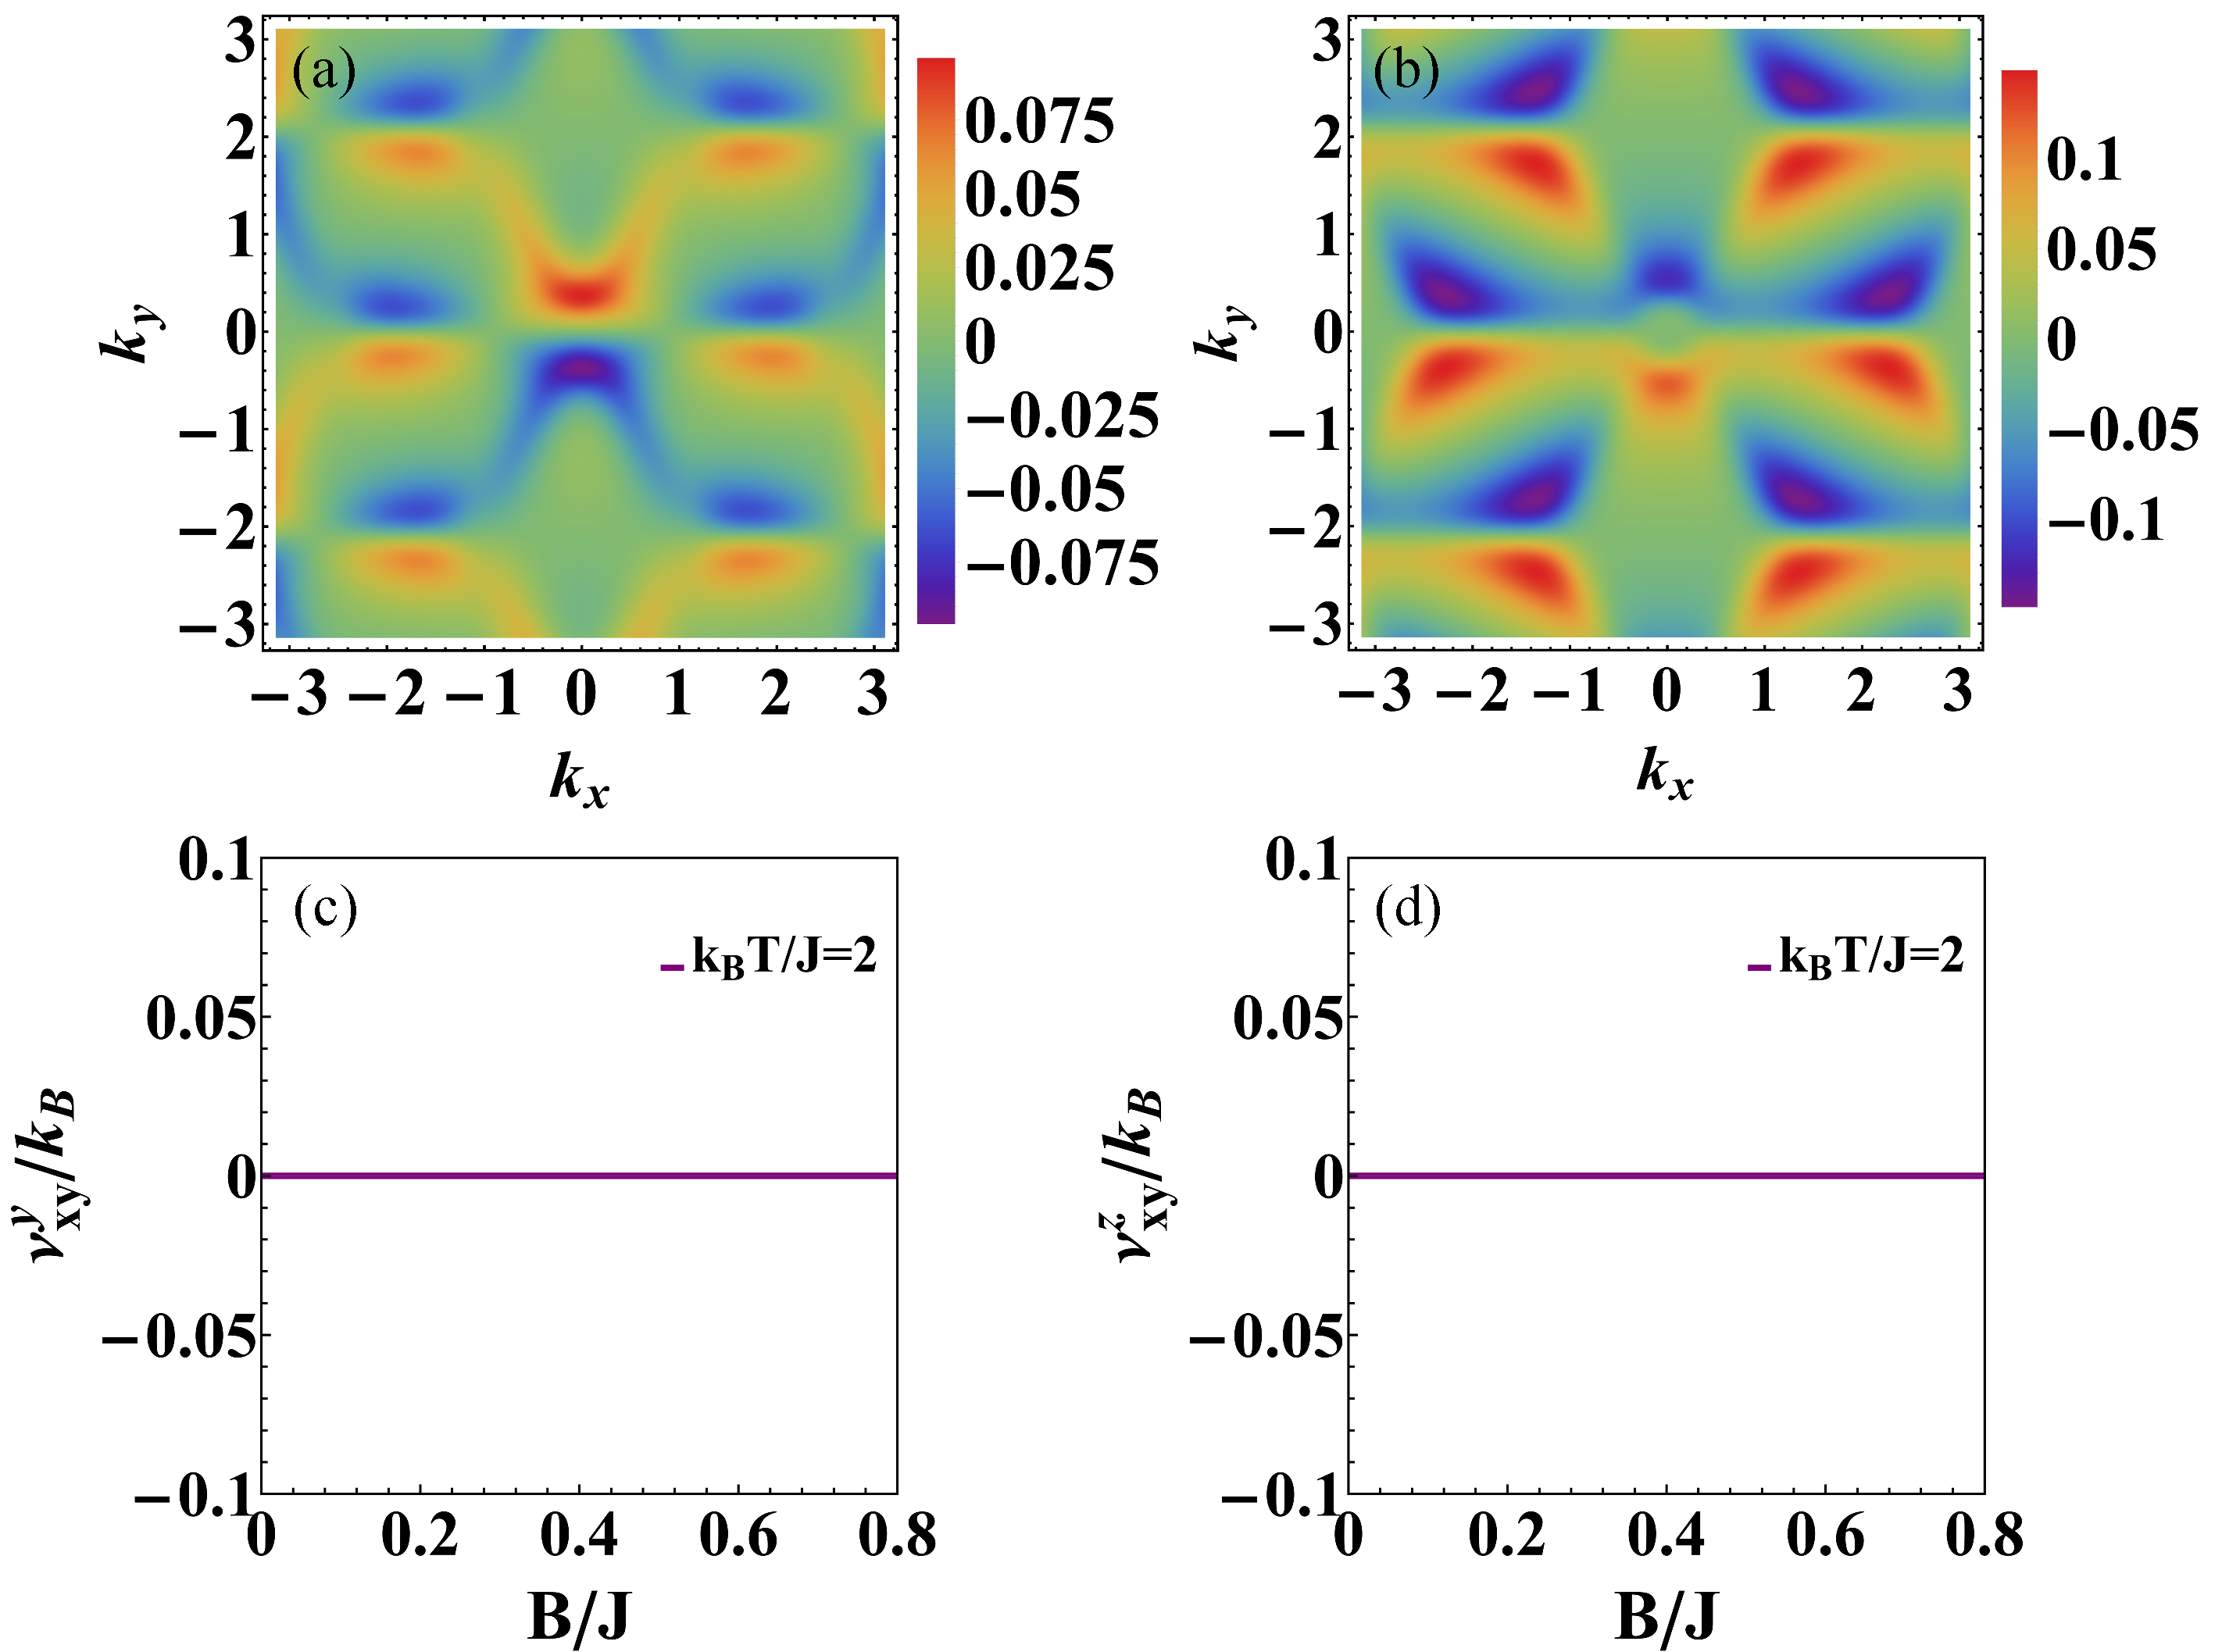
\includegraphics[width=0.88\textwidth]{Fig10-Torque.pdf}
    \caption{设定参数为 $\eta/J=6, D/J=0.06, B/J=0.6$。(a) 为自旋方向 $s=y$ 时力矩项的广义Berry曲率图，展示的是第一能带的情况。(b) 为自旋方向 $s=z$ 时第一能带的广义 Berry 曲率图。(c) 和 (d) 分别展示了系数 $\nu^y_{xy}$和$\nu^z_{xy}$ 随温度的变化，这些系数实际上均为零。图片来自~\cite{lu2024Spin}。}
    \label{fig:Torque}
\end{figure}

图\ref{fig:Torque}(a)和\ref{fig:Torque}(b)表明力矩项的广义Berry曲率 $(\tilde{\symup{\Omega}}_T)^s_{\alpha,n{\bm{k}}}$ 确实满足关系 $(\tilde{\symup{\Omega}}_T)^s_{\alpha,n{\bm{k}}}=-(\tilde{\symup{\Omega}}_T)^s_{\alpha,n(\bm{-k})}$。图~\ref{fig:Torque}(c)和\ref{fig:Torque}(d)则显示该系数为零。


% 后置部分包含参考文献、声明页（自动生成）等
\backmatter

% 打印参考文献列表
\printbibliography

\chapter{硕士期间论文发表情况}
\begin{enumerate}
  \item \underline{Bowen Lu}, Bowen Ma, Yue Yu, and Gang Chen. Spin Nernst effects of linear flavor-waves in quantum  paramagnets. \emph{Physical Review B}, 2024, \textbf{110}(23): 235109. DOI: \href{https://doi.org/10.1103/PhysRevB.110.235109}{10.1103/PhysRevB.110.235109}.

\end{enumerate}

\begin{acknowledgements}
  事情的发展，出人意料，但又在情理之中。我规划好了每一步的道路，却总是让其停留在想法，而没有付诸实践。

  在复旦的这段时间，就像做梦一样，恍惚而又真实。没想到转眼就到了终点。回想本科的致谢，我好像也是这样，似乎我总是留下一堆的遗憾，没有完成。

  感谢我的老师虞跃教授和陈钢教授。虞跃老师非常和蔼可亲，在学术上给了我很多有益的指导。陈钢老师虽不在复旦，但是通过线上的交流，也给了我很多的帮助。感谢来复旦访问时认识的吴咏时老师，吴老师平易近人，我们经常一起散步，聊了很多有意思的话题，吴老师给我写了很多推荐信，但是我的原因，没能顺利出国。也许我很让老师们失望吧，其实一直错失了很多很好的机会。还有非常多的老师，在此一并感谢你们提供的帮助。

  感谢马博文师兄，非常巧，可以遇到一个同名的师兄。在科研的道路上，他给我了非常多的帮助，感谢师兄经常在深夜与我讨论问题，带领我一步步完成这个课题，对我的很多细碎、繁琐的问题，师兄总是耐心给予我解答。

  感谢高永豪师兄和刘剑翘师姐，在我科研初期，你们给予了我很多的帮助，高永豪师兄带领我进入的科研的大门，解决了我很多的基础问题和困惑，刘剑翘师姐在后来和我进行了非常多的讨论，帮我进行了很多繁杂的推导，帮我检查我的程序问题，让我慢慢可以做一些科研工作，师姐的耐心教导给我受益颇多。感谢张乃维老师，在我刚进复旦时候，给了我很多生活上的支持，帮我解决了很多困难，也给我提供了非常多的关照，让我可以融入复旦的生活。感谢刘长乐师兄，我很晚才认识刘师兄，但师兄积极乐观，和师兄交流非常有趣，师兄也给我说了很多他人生的经历和建议，让我受益良多，希望师兄的身体可以逐渐好转，可以碰上好的人生机遇。同时也要感谢李朝恺师兄、姚旭平师兄、黄春炯师兄，给了我很多课题和很多有意的讨论，但我效率太低，大多都没有完成。

  感谢课题组的詹烨旻师姐，师姐非常活泼乐观，和她的交流总是轻松而愉悦，师姐也对我非常关心，在我迷茫的时候给予我很多鼓励，在我困难时给予了很多帮助，平时也会时常关心我的科研近况，不甚感激。

  同时也要感谢课题组的罗熙师兄，陈宇戈师兄，马迪师兄，毛冠东师兄，感谢平时和他们有意的讨论，不只是课题方面，还有生活方面。马迪师兄总是邀请我一同出去游玩，和我交流他的思想和看法，给予了我非常多的帮助。

  感谢我的室友，詹研，徐一翔，杨中元。研一刚开学的时候，我们的见面还历历在目，我们本是直博，将会一起离开，但是我成为了最先离开的那个。很巧的是，我们四个都是党员，于是我们的宿舍名变为了“12\_701党支部”，而我们都以书记相称，詹书记，杨书记，卢书记，徐书记，而徐书记这个称呼在后来，慢慢演化成了翔哥。感谢詹书记在答辩后给我送的花，感谢翔哥特地从邯郸回来和我拍合照，并给我拍了很多精美的照片，杨书记没有赶上校车，非常遗憾。

  感谢S519的欧阳创新、王昱天、杜学瑞、丁朝阳、王炯杰、刘泽宇、张硕、王浩铖、成行等朋友们，我们经常一起吃饭，一起出去玩，毕业一块聚餐，一块交流问题，很高兴可以一起玩耍。

  感谢学工组的老师们，唐诗蕊老师、闫晓辉老师、许蓓蕾老师、肖文老师，还有之前的辅导员，董树婷、楚娇，在学习生活中有非常多的琐事，你们都给予了耐心的解答，也给我提供了非常多的信息和帮助，非常感谢。

  还有黄泽宇，感谢你在我迷茫的时候一直约我出去吃饭，并和我散步聊天，和我聊一些你对未来的学业和生活的规划，让我非常受益。感谢殷林琪院士，你让我感受到了本科生的活力，和你的聊天总是让我心情很好。还有洪梓敬，我们讨论了很多物理、篮球相关的话题。

  还有太多太多朋友，特别是那些在我困难时给我提供了帮助的朋友们，非常感谢你们能伸出援手，拯救我于水火之中，恕我无法在此一一提及你们的姓名，但我会永远记得和你们度过的欢乐时光。

  我到底是一个什么样的人呢？我也不知道，我知道很多事我需要去做，我有理想，有想要完成的事，但我迟迟无法动手，我总是在拖延，这是逃避吗？可能是吧，因为无法把任务做好，所以就逃避去做，只躺在自己的舒适区圈，甚至不在舒适圈，不过是虚度光阴，空度年华。就像本篇致谢，在最后一天才迟迟开始动笔……

  我真的有很多朋友吗？我确实认识非常多的人，但是多少可以称为朋友，多少只是认识呢？

  我已经陷入焦虑，有太多的事我不知，有太多的事需要我去解决，有太多的事我无法掌握。我是一个积极的人，还是一个消极的人？这些内容应该出现在致谢里吗？写上这些内容，以后你会改变吗？我不知道。

  转眼已经26岁了，多去尝试吧，多去失败吧，多去经历吧，多去面对吧。生活在真实的世界中，而不是活在梦中。

  应该会有答案的，应该会有的。

  \begin{flushright}
    卢博文 \\
    于复旦大学江湾校区物理楼S519工位前\\
    2025年5月26日\\
  \end{flushright}
\end{acknowledgements}

\end{document}